
\begin{frame}[t]\frametitle{Búsquedas geolocalizadas}

La búsqueda geolocalizada es una herramienta que nos da la posibilidad de obtener tuits generados en un área geográfica particular. Para esto, primero intenta buscar tuits cuyas coordenadas sean las buscadas.


\begin{columns}
    \begin{column}{0.33\textwidth}
        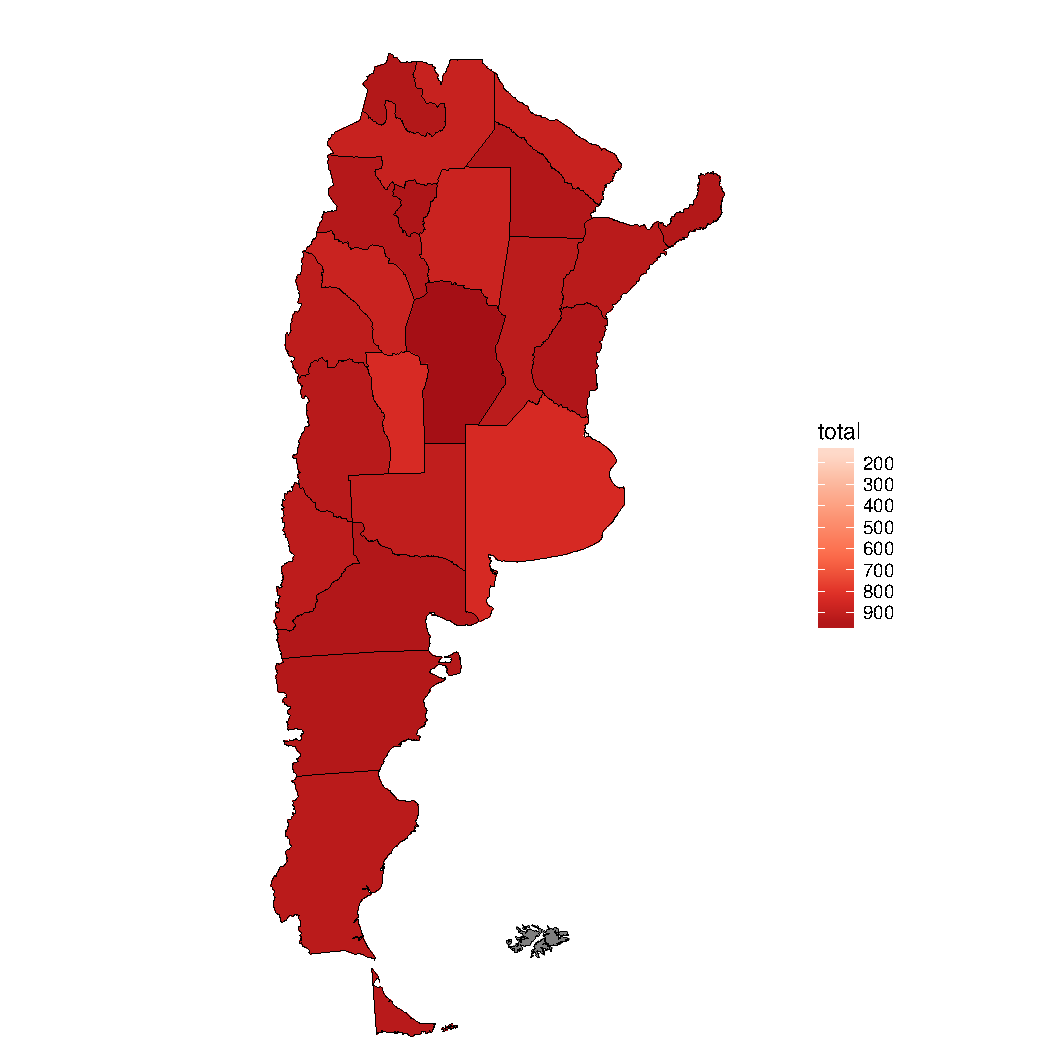
\includegraphics[width=\linewidth]{../src/images/mapaprovincias.pdf}
        \caption{} 
        \label{fig:mapaProvincias}
    \end{column}

    \begin{column}{0.33\textwidth}
        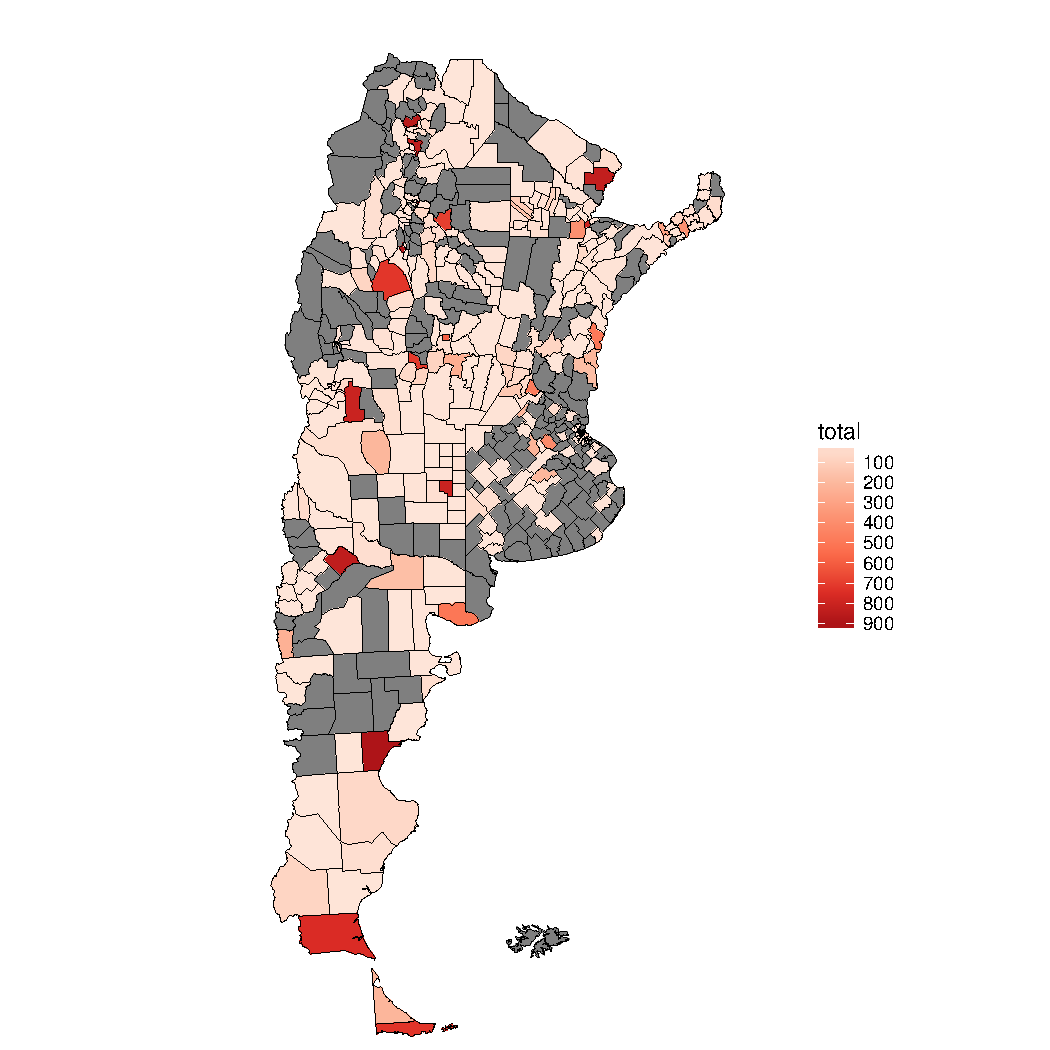
\includegraphics[width=\linewidth]{../src/images/mapadepartamentos.pdf}
        \caption{} 
        \label{fig:mapaDepartamentos}
    \end{column}

    \begin{column}{0.33\textwidth}
        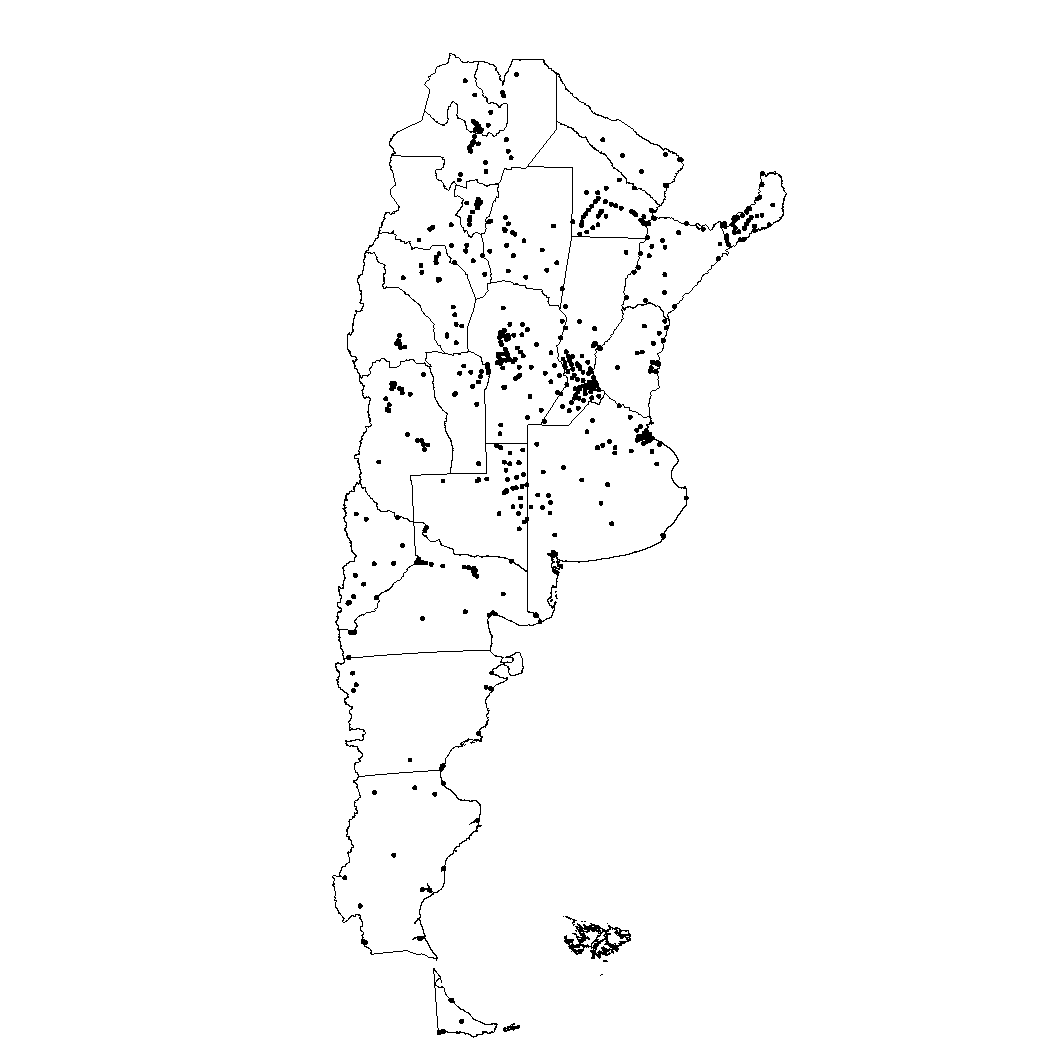
\includegraphics[width=\linewidth]{../src/images/mapaprovinciasConPuntos.pdf}
    \caption{} 
    \label{fig:mapaPuntos}
    \end{column}

\end{columns}

Se realizaron búsquedas por cada provincia con centro en las coordenadas de los departamentos de la misma y con un radio de 20 millas. 

Nos quedamos con los usuarios que tienen como campo \textit{location} al menos uno de los nombres de las ciudades de la provincia. 



\end{frame}



% \begin{figure}[!ht]\centering
%   \begin{subfigure}[t]{0.20\textwidth}
%     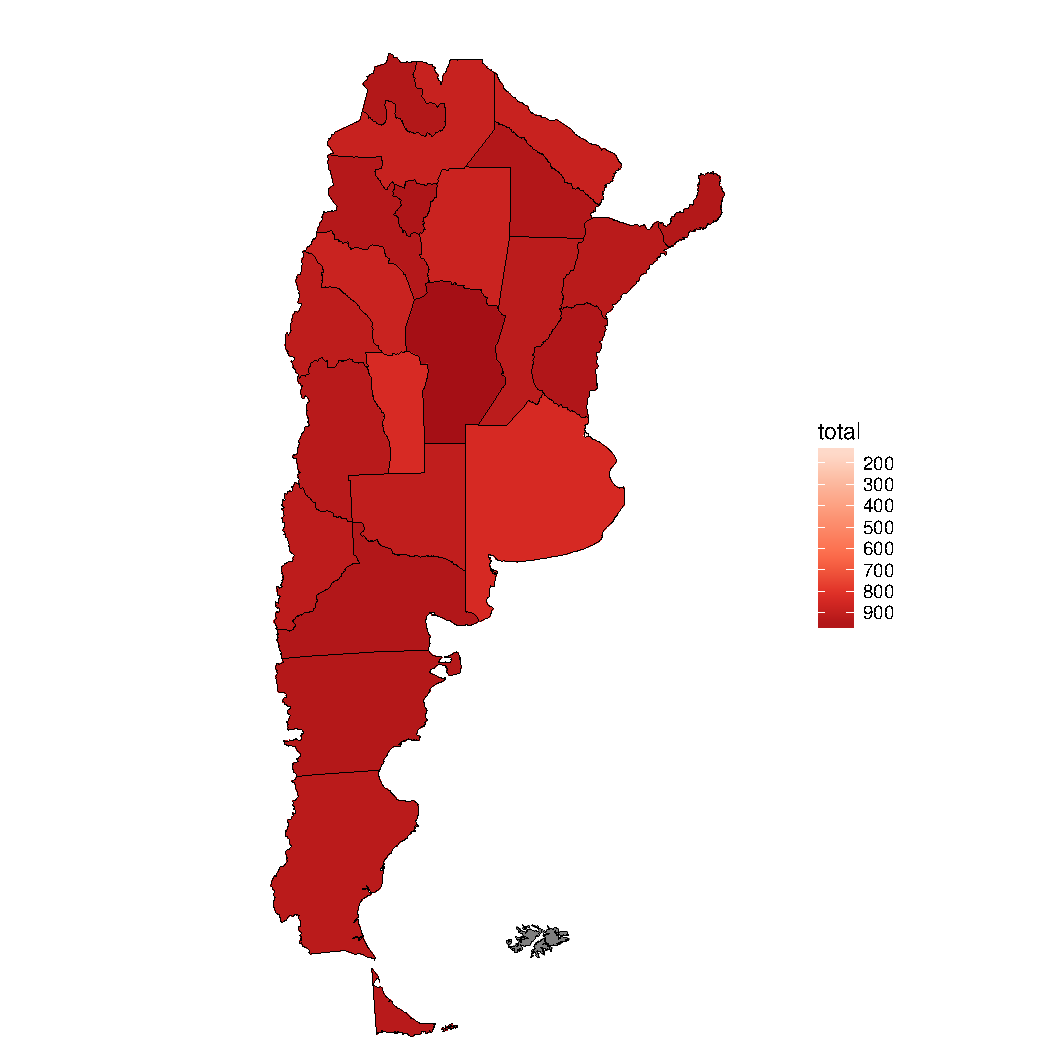
\includegraphics[width=\linewidth]{../src/images/mapaprovincias.pdf}
%     \caption{} 
%     \label{fig:mapaProvincias} 
%    \end{subfigure}
%    \begin{subfigure}[t]{0.20\textwidth}
%     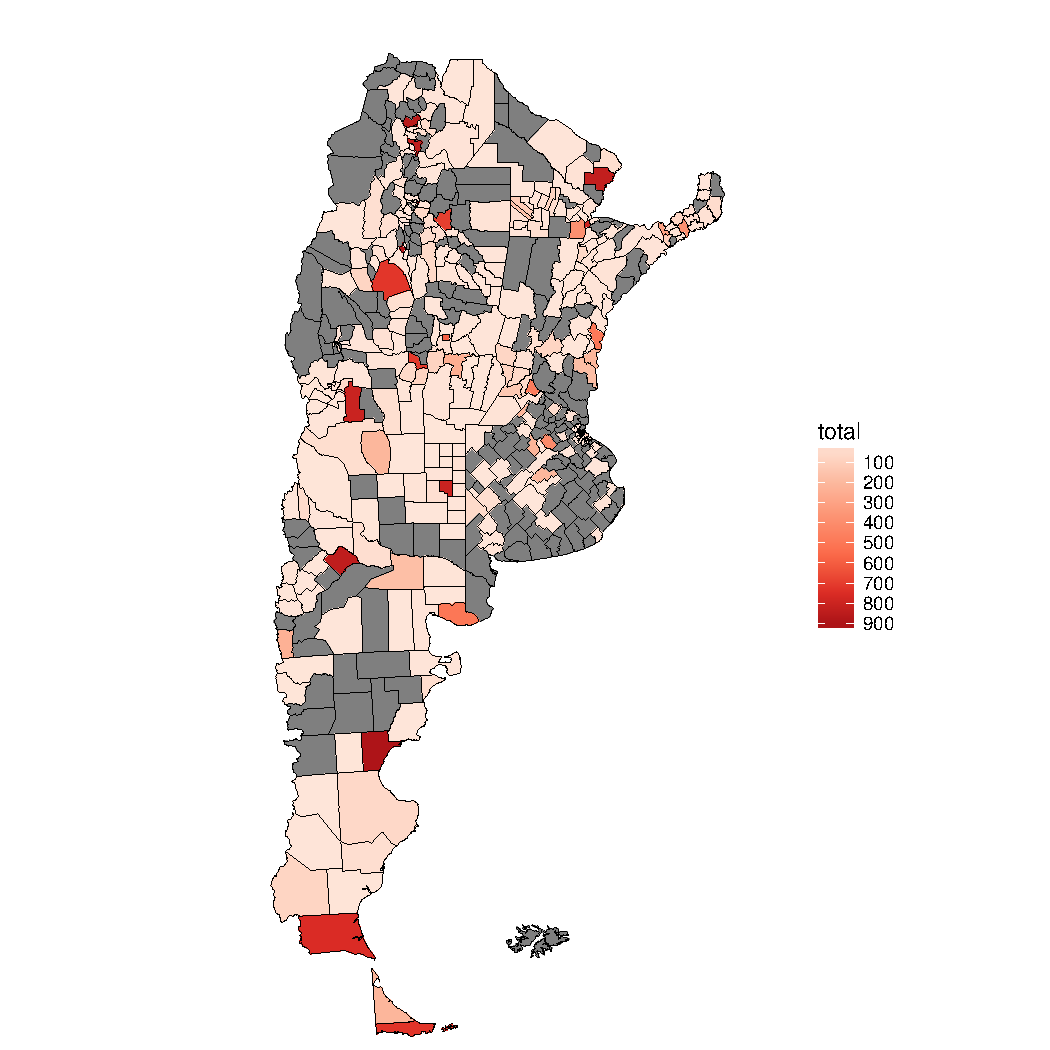
\includegraphics[width=\linewidth]{../src/images/mapadepartamentos.pdf}
%     \caption{} 
%     \label{fig:mapaDepartamentos} 
%    \end{subfigure}
%    \begin{subfigure}[t]{0.20\textwidth}
%     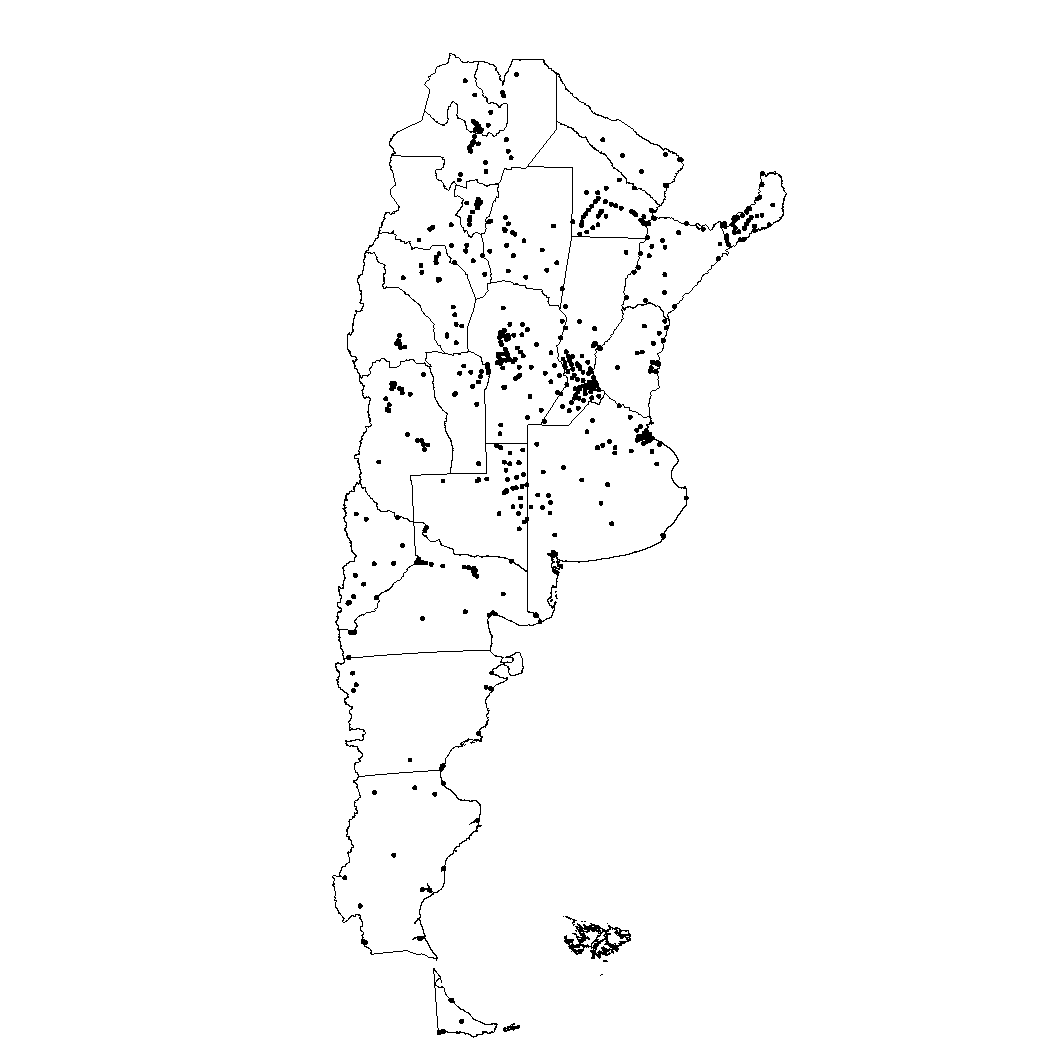
\includegraphics[width=\linewidth]{../src/images/mapaprovinciasConPuntos.pdf}
%     \caption{} 
%     \label{fig:mapaPuntos} 
%    \end{subfigure}    
% \end{figure}

